%
% 23-mathpendel.tex -- Das mathematische Pendel
%
% (c) 2022 Prof Dr Andreas Müller, OST Ostschweizer Fachhochschule
%

\subsection{Das mathematische Pendel
\label{buch:elliptisch:subsection:mathpendel}}
\begin{figure}
\centering
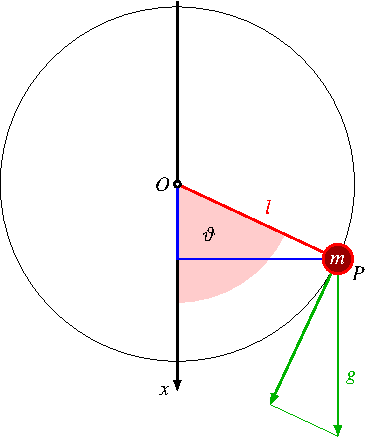
\includegraphics{chapters/110-elliptisch/images/pendel.pdf}
\caption{Mathematisches Pendel
\label{buch:elliptisch:fig:mathpendel}}
\end{figure}
Das in Abbildung~\ref{buch:elliptisch:fig:mathpendel} dargestellte
mathematische Pendel besteht aus einem Massepunkt der Masse $m$
im Punkt $P$,
der über eine masselose Stange der Länge $l$ mit dem Drehpunkt $O$
verbunden ist.
Das Pendel bewegt sich unter dem Einfluss der Schwerebeschleunigung $g$.

Das Trägheitsmoment des Massepunktes um den Drehpunkt $O$ ist
\(
I=ml^2
\).
Das Drehmoment der Schwerkraft ist
\(M=gl\sin\vartheta\).
Die Bewegungsgleichung wird daher
\[
\begin{aligned}
\frac{d}{dt} I\dot{\vartheta}
&=
M
=
gl\sin\vartheta
\\
ml^2\ddot{\vartheta}
&=
gl\sin\vartheta
&&\Rightarrow&
\ddot{\vartheta}
&=\frac{g}{l}\sin\vartheta.
\end{aligned}
\]
Dies ist eine nichtlineare Differentialgleichung zweiter Ordnung, die
wir nicht unmittelbar mit den Differentialgleichungen erster Ordnung
der elliptischen Funktionen vergleichen können.

Die Differentialgleichungen erster Ordnung der elliptischen Funktionen
enthalten das Quadrat der ersten Ableitung.
In unserem Fall entspricht das einer Gleichung, die $\dot{\vartheta}^2$
enthält.
Der Energieerhaltungssatz kann uns eine solche Gleichung geben.
Die Summe von kinetischer und potentieller Energie muss konstant sein.
Dies führt auf
\begin{equation}
E_{\text{kinetisch}}
+
E_{\text{potentiell}}
=
\frac12I\dot{\vartheta}^2
+
mgl(1-\cos\vartheta)
=
\frac12ml^2\dot{\vartheta}^2
+
mgl(1-\cos\vartheta)
=
E.
\label{buch:elliptisch:mathpendel:energiegleichung}
\end{equation}
Durch Auflösen nach $\dot{\vartheta}$ kann man jetzt die
Differentialgleichung
\[
\dot{\vartheta}^2
=
-
\frac{2g}{l}(1-\cos\vartheta)
+\frac{2E}{ml^2}
\]
finden.
In erster Näherung, d.h. wenn man die rechte Seite bis zu vierten
Potenzen in eine Taylor-Reihe in $\vartheta$ entwickelt,  ist dies
tatsächlich eine Differentialgleichung der Art, wie wir sie für
elliptische Funktionen gefunden haben, wir möchten aber eine exakte
Lösung konstruieren.

Die maximale Energie für eine Bewegung, bei der sich das Pendel gerade
über den höchsten Punkt hinweg zu bewegen vermag, ist 
$E=2lmg$.
Falls $E<2mgl$ ist, erwarten wir Schwingungslösungen, bei denen 
der Winkel $\vartheta$ immer im offenen Interval $(-\pi,\pi)$
bleibt.
Für $E>2mgl$ wird sich das Pendel im Kreis bewegen, für sehr grosse
Energie ist die kinetische Energie dominant, die Verlangsamung im
höchsten Punkt wird immer weniger ausgeprägt sein.


%
% Koordinatentransformation auf elliptische Funktionen
%
\subsubsection{Koordinatentransformation auf elliptische Funktionen}
Wir verwenden als neue Variable 
\begin{align}
y
&=
\sin\frac{\vartheta}2
&&\Rightarrow&
\cos^2\frac{\vartheta}2
&=
1-y^2.
\label{buch:elliptisch:mathpendel:ydef}
\intertext{Die Ableitung ist}
\dot{y}
&=
\frac12\cos\frac{\vartheta}{2}\cdot \dot{\vartheta}
&&\Rightarrow&
\dot{y}^2
&=
\frac14\cos^2\frac{\vartheta}2\cdot\dot{\vartheta}^2.
\label{buch:elliptisch:mathpendel:yabl}
\intertext{%
Man beachte, dass die Koordinate senkrecht zur $x$-Achse in 
Abbildung~\ref{buch:elliptisch:fig:mathpendel} die Auslenkung
$l\sin\vartheta$ ist, $y$ ist also nicht die Auslenkung senkrecht
zur $x$-Achse!
Aus den Halbwinkelformeln finden wir ausserdem
}
\cos\vartheta
&=
1-2\sin^2 \frac{\vartheta}2
=
1-2y^2
&&\Rightarrow&
1-\cos\vartheta
&=
2y^2.
\label{buch:elliptisch:mathpendel:halbwinkel}
\end{align}
Die Grösse $1-\cos\vartheta$ haben wir in der Energiegleichung
\eqref{buch:elliptisch:mathpendel:energiegleichung}
bereits angetroffen.

Die Identitäten 
\eqref{buch:elliptisch:mathpendel:halbwinkel}
%und
%\eqref{buch:elliptisch:mathpendel:ydef}
können wir jetzt in die
Energiegleichung~\eqref{buch:elliptisch:mathpendel:energiegleichung}
einsetzen und erhalten
\begin{align}
\frac12ml^2\dot{\vartheta}^2 + 2mgly^2
&=
E
\intertext{und nach Division durch $2ml^2$}
\frac14 \dot{\vartheta}^2
&=
\frac{E}{2ml^2} - \frac{g}{l}y^2.
\label{buch:elliptisch:mathpendel:thetadgl}
\end{align}
%Der konstante Term auf der rechten Seite ist grösser oder kleiner als
%$1$ je nachdem, ob das Pendel sich im Kreis bewegt oder nicht.
Durch Multiplizieren mit der rechten Gleichung von
\eqref{buch:elliptisch:mathpendel:ydef}
erhalten wir auf der linken Seite einen Ausdruck, den wir
mit Hilfe von \eqref{buch:elliptisch:mathpendel:yabl}
als Funktion von $\dot{y}$ ausdrücken können.
Wir erhalten
\begin{align}
\underbrace{\frac14
\cos^2\frac{\vartheta}2
\cdot
\dot{\vartheta}^2}_{\displaystyle=\dot{y}^2}
&=
(1-y^2)
\biggl(\frac{E}{2ml^2} -\frac{g}{l}y^2\biggr)
\notag
\\
\dot{y}^2
&=
(1-y^2)
\biggl(\frac{E}{2ml^2} -\frac{g}{l}y^2\biggr).
\label{buch:elliptisch:mathpendel:ydgl}
\end{align}
Die letzte Gleichung hat die Form einer Differentialgleichung
für elliptische Funktionen.
Welche Funktion verwendet werden muss, hängt von der relativen
Grösse der Koeffizienten in der zweiten Klammer ab.

%
% Zeittransformation zur Elimination des konstanten Faktors
%
\subsubsection{Zeittransformation}
Die Gleichung~\eqref{buch:elliptisch:mathpendel:ydgl} kann auch in
die Form
\begin{equation}
\frac{2ml^2}{E}\dot{y}^2
=
(1-y^2)\biggl(1-\frac{2mgl}{E}y^2\biggr)
\label{buch:elliptisch:mathpendel:ydgl2}
\end{equation}
gebracht werden.
Der konstante Faktor auf der linken Seite kann wie in der Diskussion
des anharmonischen Oszillators durch eine lineare
Transformation der Zeit zum Verschwinden gebracht werden.
Dazu setzt man $z(t) = y(bt)$ und bekommt
\[
\frac{d}{dt}z(t)
=
\frac{d}{dt}y(bt) \frac{d\,bt}{dt}
=
b\,\dot{y}(bt).
\]
Die Zeit muss also mit dem Faktor $\sqrt{2ml^2/E}$ skaliert werden.

%
% Nullstellen der rechten Seite der Differentialgleichung
%
\subsubsection{Nullstellen der rechten Seite}
Die rechte Seite von \eqref{buch:elliptisch:mathpendel:ydgl2}
hat die beiden Nullstellen $1$ und
\begin{equation}
y_0=\sqrt{\frac{E}{2mgl}}. 
\label{buch:elliptisch:mathpendel:y0}
\end{equation}
Die Differentialgleichung kann damit als
\begin{equation}
\dot{y}^2
=
(1-y^2)\biggl(1-\frac{1}{y_0^2}y^2\biggr)
\label{buch:elliptisch:mathpendel:y0dgl}
\end{equation}
geschrieben werden.
Da die linke Seite $\ge 0$ sein muss, muss 
\(
y\le \min(1,y_0)
\)
sein.
Damit ergeben sich zwei Fälle.
Wenn $y_0<1$ ist, dann schwingt das Pendel.
Der Fall $y_0>1$ entspricht einer Bewegung, bei der das Pendel
um den Punkt $O$ rotiert.
In den folgenden zwei Abschnitten werden die beiden Fälle ausführlicher
diskutiert.


\begin{figure}
\centering
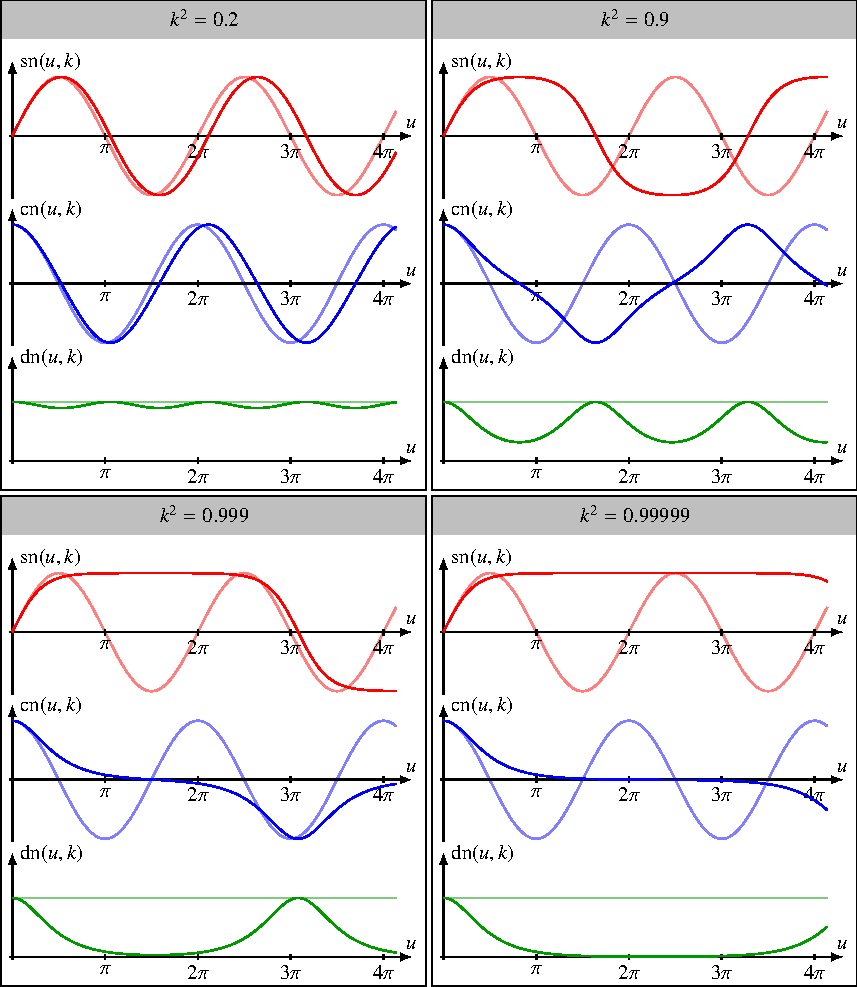
\includegraphics[width=\textwidth]{chapters/110-elliptisch/images/jacobiplots.pdf}
\caption{%
Abhängigkeit der elliptischen Funktionen von $u$ für
verschiedene Werte von $k^2=m$.
Für $m=0$ ist $\operatorname{sn}(u,0)=\sin u$, 
$\operatorname{cn}(u,0)=\cos u$ und $\operatorname{dn}(u,0)=1$, diese
sind in allen Plots in einer helleren Farbe eingezeichnet.
Für kleine Werte von $m$ weichen die elliptischen Funktionen nur wenig
von den trigonometrischen Funktionen ab,
es ist aber klar erkennbar, dass die anharmonischen Terme in der
Differentialgleichung die Periode mit steigender Amplitude verlängern.
Sehr grosse Werte von $m$ nahe bei $1$ entsprechen der Situation, dass
die Energie des Pendels fast ausreicht, dass es den höchsten Punkt
erreichen kann, was es für $m$ macht.
\label{buch:elliptisch:fig:jacobiplots}}
\end{figure}

\subsubsection{Der Fall $E>2mgl$}
In diesem Fall ist die zweite Nullstelle $y_0>1$ oder $1/y_0^2 < 1$.
Die Differentialgleichung~\eqref{buch:elliptisch:mathpendel:y0dgl}
sieht ganz ähnlich aus wie die Differentialgleichung der
Funktion $\operatorname{sn}(u,k)$, tatsächlich wird sie zur
Differentialgleichung von $\operatorname{sn}(u,k)$ wenn man
\[
k^2
=
1/y_0^2
=
\frac{2mgl}{E}
\]
wählt.
In diesem Fall ist also $y=\operatorname{sn}(u,1/y_0)$ eine Lösung
der Differentialgleichung, wobei $u$ eine lineare Funktion der Zeit
ist.

Wenn $y_0 \gg 1$ ist, dann ist $k\approx 0$ und die Bewegung ist
entspricht einer gleichförmigen Kreisbewegung.
Je näher $y_0$ an $1$ liegt, desto näher an $1$ ist auch $k$ und
desto grösser wird die Verlangsamung der Bewgung in der Nähe des
Scheitels, das Pendel verweilt sehr lange.
Dies äussert sich in Abbildung~\ref{buch:elliptisch:fig:jacobiplots}
durch die lange Verweildauer der Funktion nahe der Extrema.

%
% Der Fall E < 2mgl
%
\subsubsection{Der Fall $E<2mgl$}
In diesem Fall ist $y_0<1$ und die
Differentialgleichung~\eqref{buch:elliptisch:mathpendel:y0dgl}
sieht zwar immer noch wie eine Differentialgleichung für
$\operatorname{sn}(u,k)$ aus, aber die Lage der Nullstellen
der rechten Seite ist verkehrt.
Indem wir $y=y_0z$ schreiben, erhalten wir 
\begin{equation}
\dot{y}^2
=
y_0^2 \dot{z}^2
=
(1-y_0^2z^2)(1-z^2).
\end{equation}
Wieder kann durch eine lineare Transformation der Zeit der Faktor $y_0^2$
auf der linken Seite zum Verschwinden gebracht werden, es bleibt
die Differentialgleichung der Funktion $\operatorname{sn}(u,k)$
mit $k=y_0$.
Daraus liest man ab, dass $y_0\operatorname{sn}(u,k)$ die Bewegung
des Pendels im oszillatorischen Fall beschreibt, wobei $u$ wieder
eine lineare Funktion der Zeit ist.

Wenn $y_0\ll 1$ ist, dann ist auch $k$ sehr klein und die lineare
Näherung ist sehr gut, das Pendel verhält sich wie ein harmonischer
Oszillator mit einer Sinus-Schwingung als Lösung.
Für $y_0=k$ nahe an $1$ dagegen erreicht die Schwingung fast den
die maximale Höhe und wird dort sehr langsam.
Dies äussert sich in Abbildung~\ref{buch:elliptisch:fig:jacobiplots}
wiederum durch die lange Verweildauer der Funktion nahe der Extrema.

